\section{Removing unreachable blocks}

There could be blocks generated in the previous pass which are \textit{unreachable}, meaning that there is no jump from
other block to those blocks. The block with \code{id} equal to \code{0} is reachable by default, since it is the entry
point of the control flow graph.

This pass scans the list of blocks and removes the blocks which are unreachable, as previously defined. The scan needs
to be repeated until there are no more blocks removed since the previous scan. This is the case because there could be
blocks which are reachable only from unreachable blocks. When the unreachable blocks are removed, these blocks become
unreachable themselves and need to be removed too.

An example of this pass is provided in \labelindexref{Figure}{img:remove-unreachable}. The block with \code{id} equal to
\code{5} is unreachable, so it gets removed in the first scan. This makes the block with \code{id} equal to \code{2}
unreachable and it gets removed in the second scan.

\begin{figure}[htb]
    \makebox[\linewidth][c]{%
    \begin{subfigure}[b]{.6\textwidth}
        \centering
        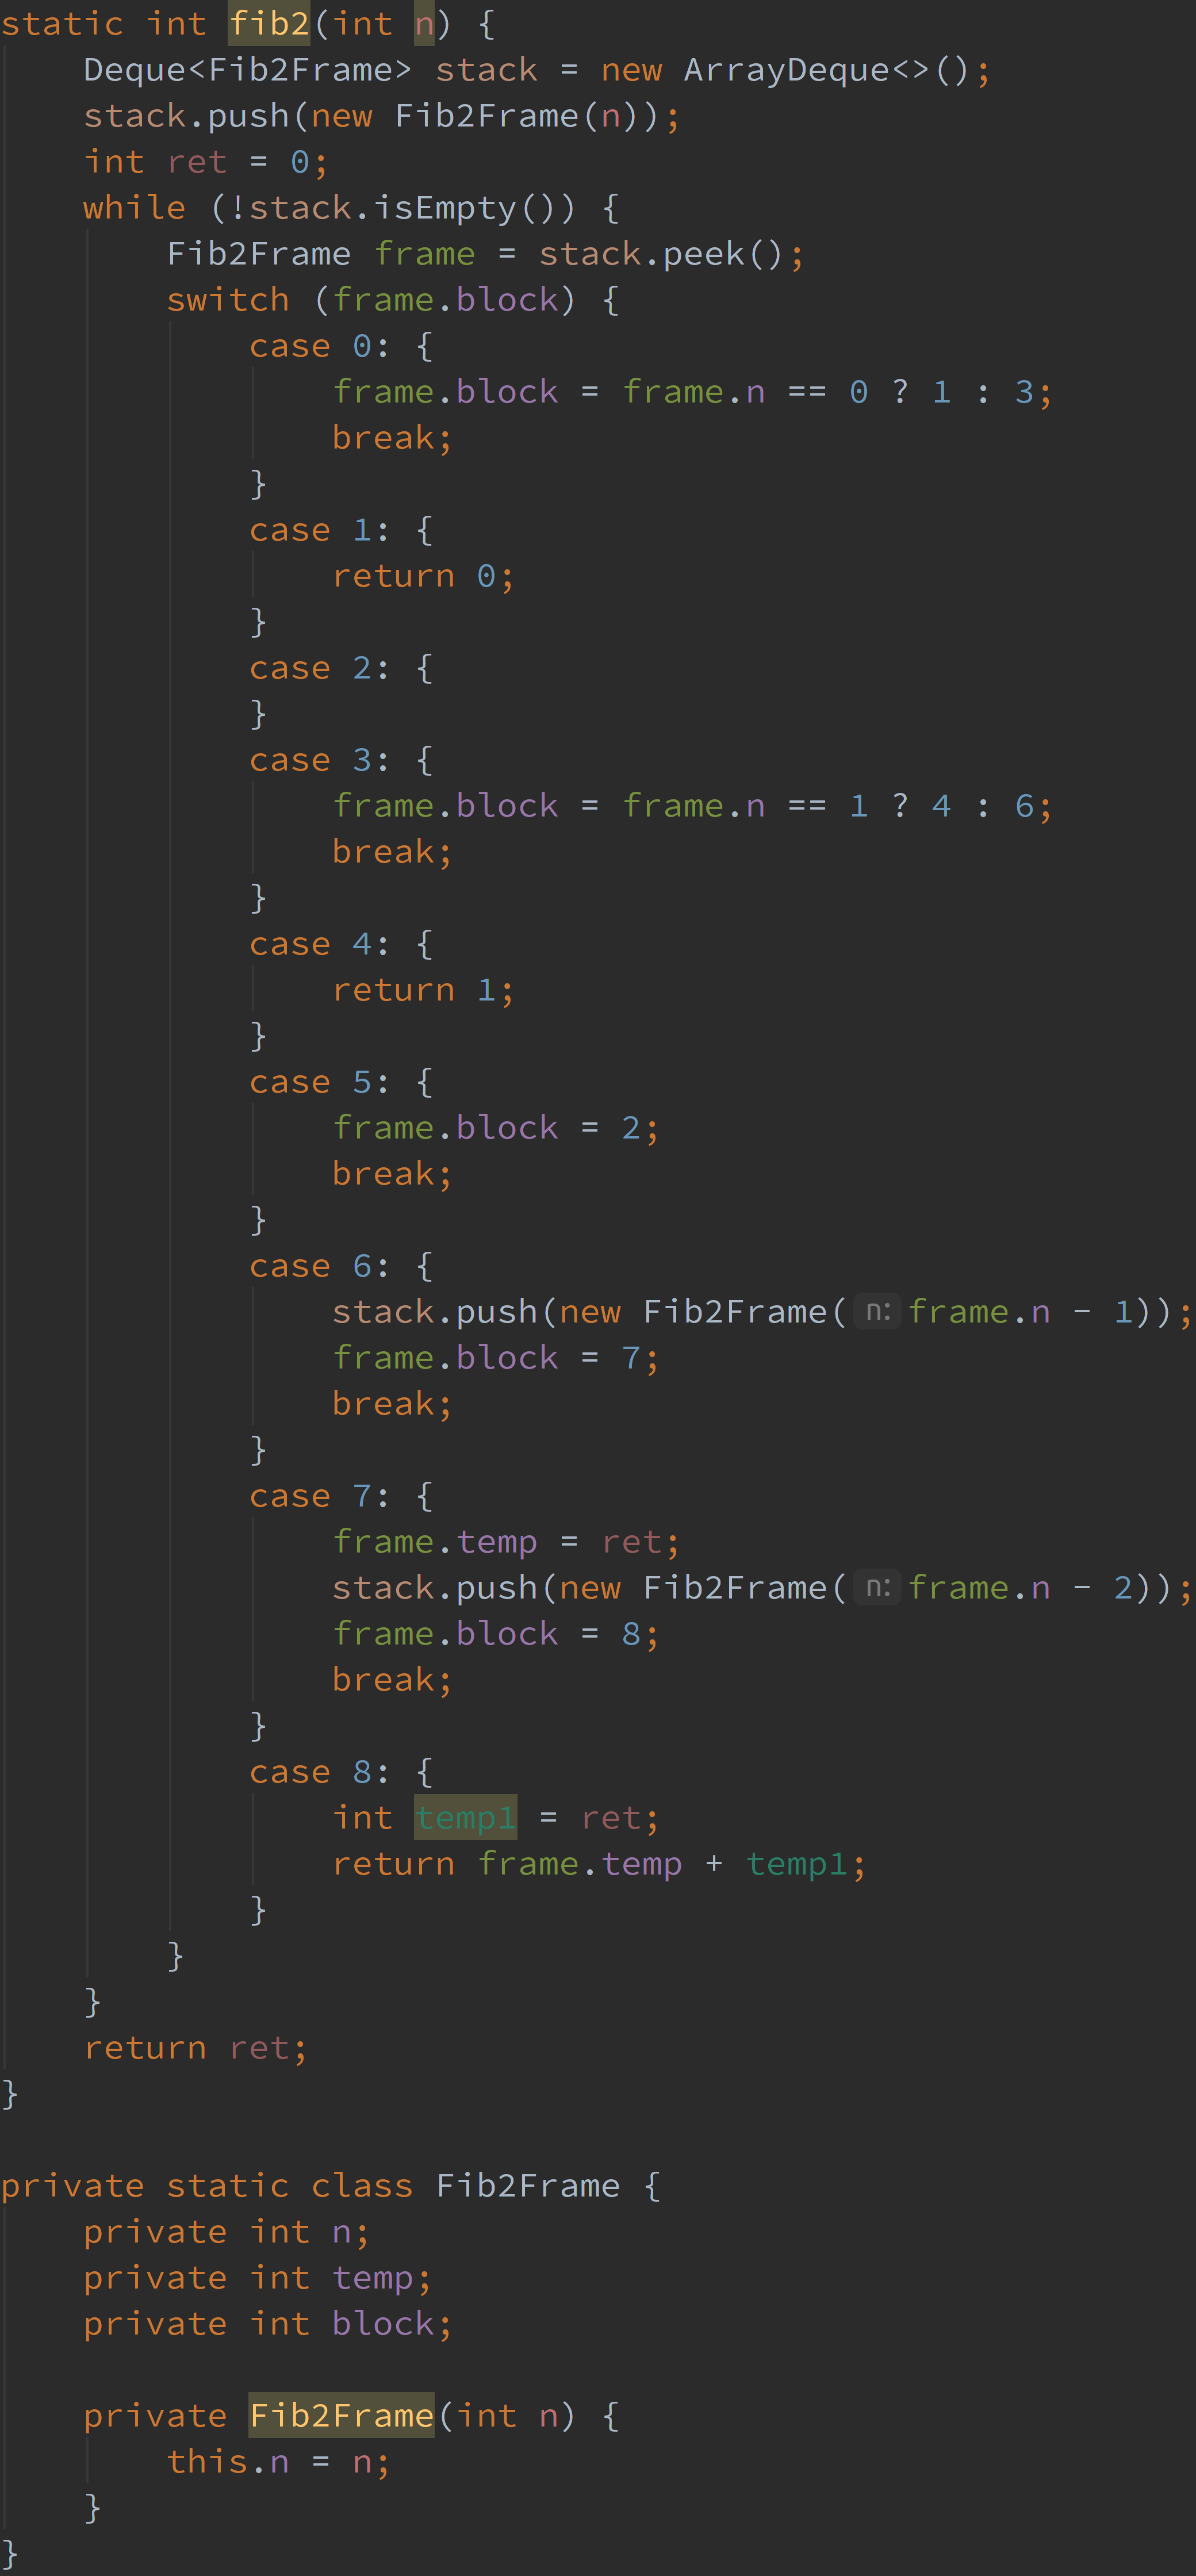
\includegraphics[height=5in]{src/img/blocks-after.png}
        \caption{Before}
    \end{subfigure}%
    \begin{subfigure}[b]{.6\textwidth}
        \centering
        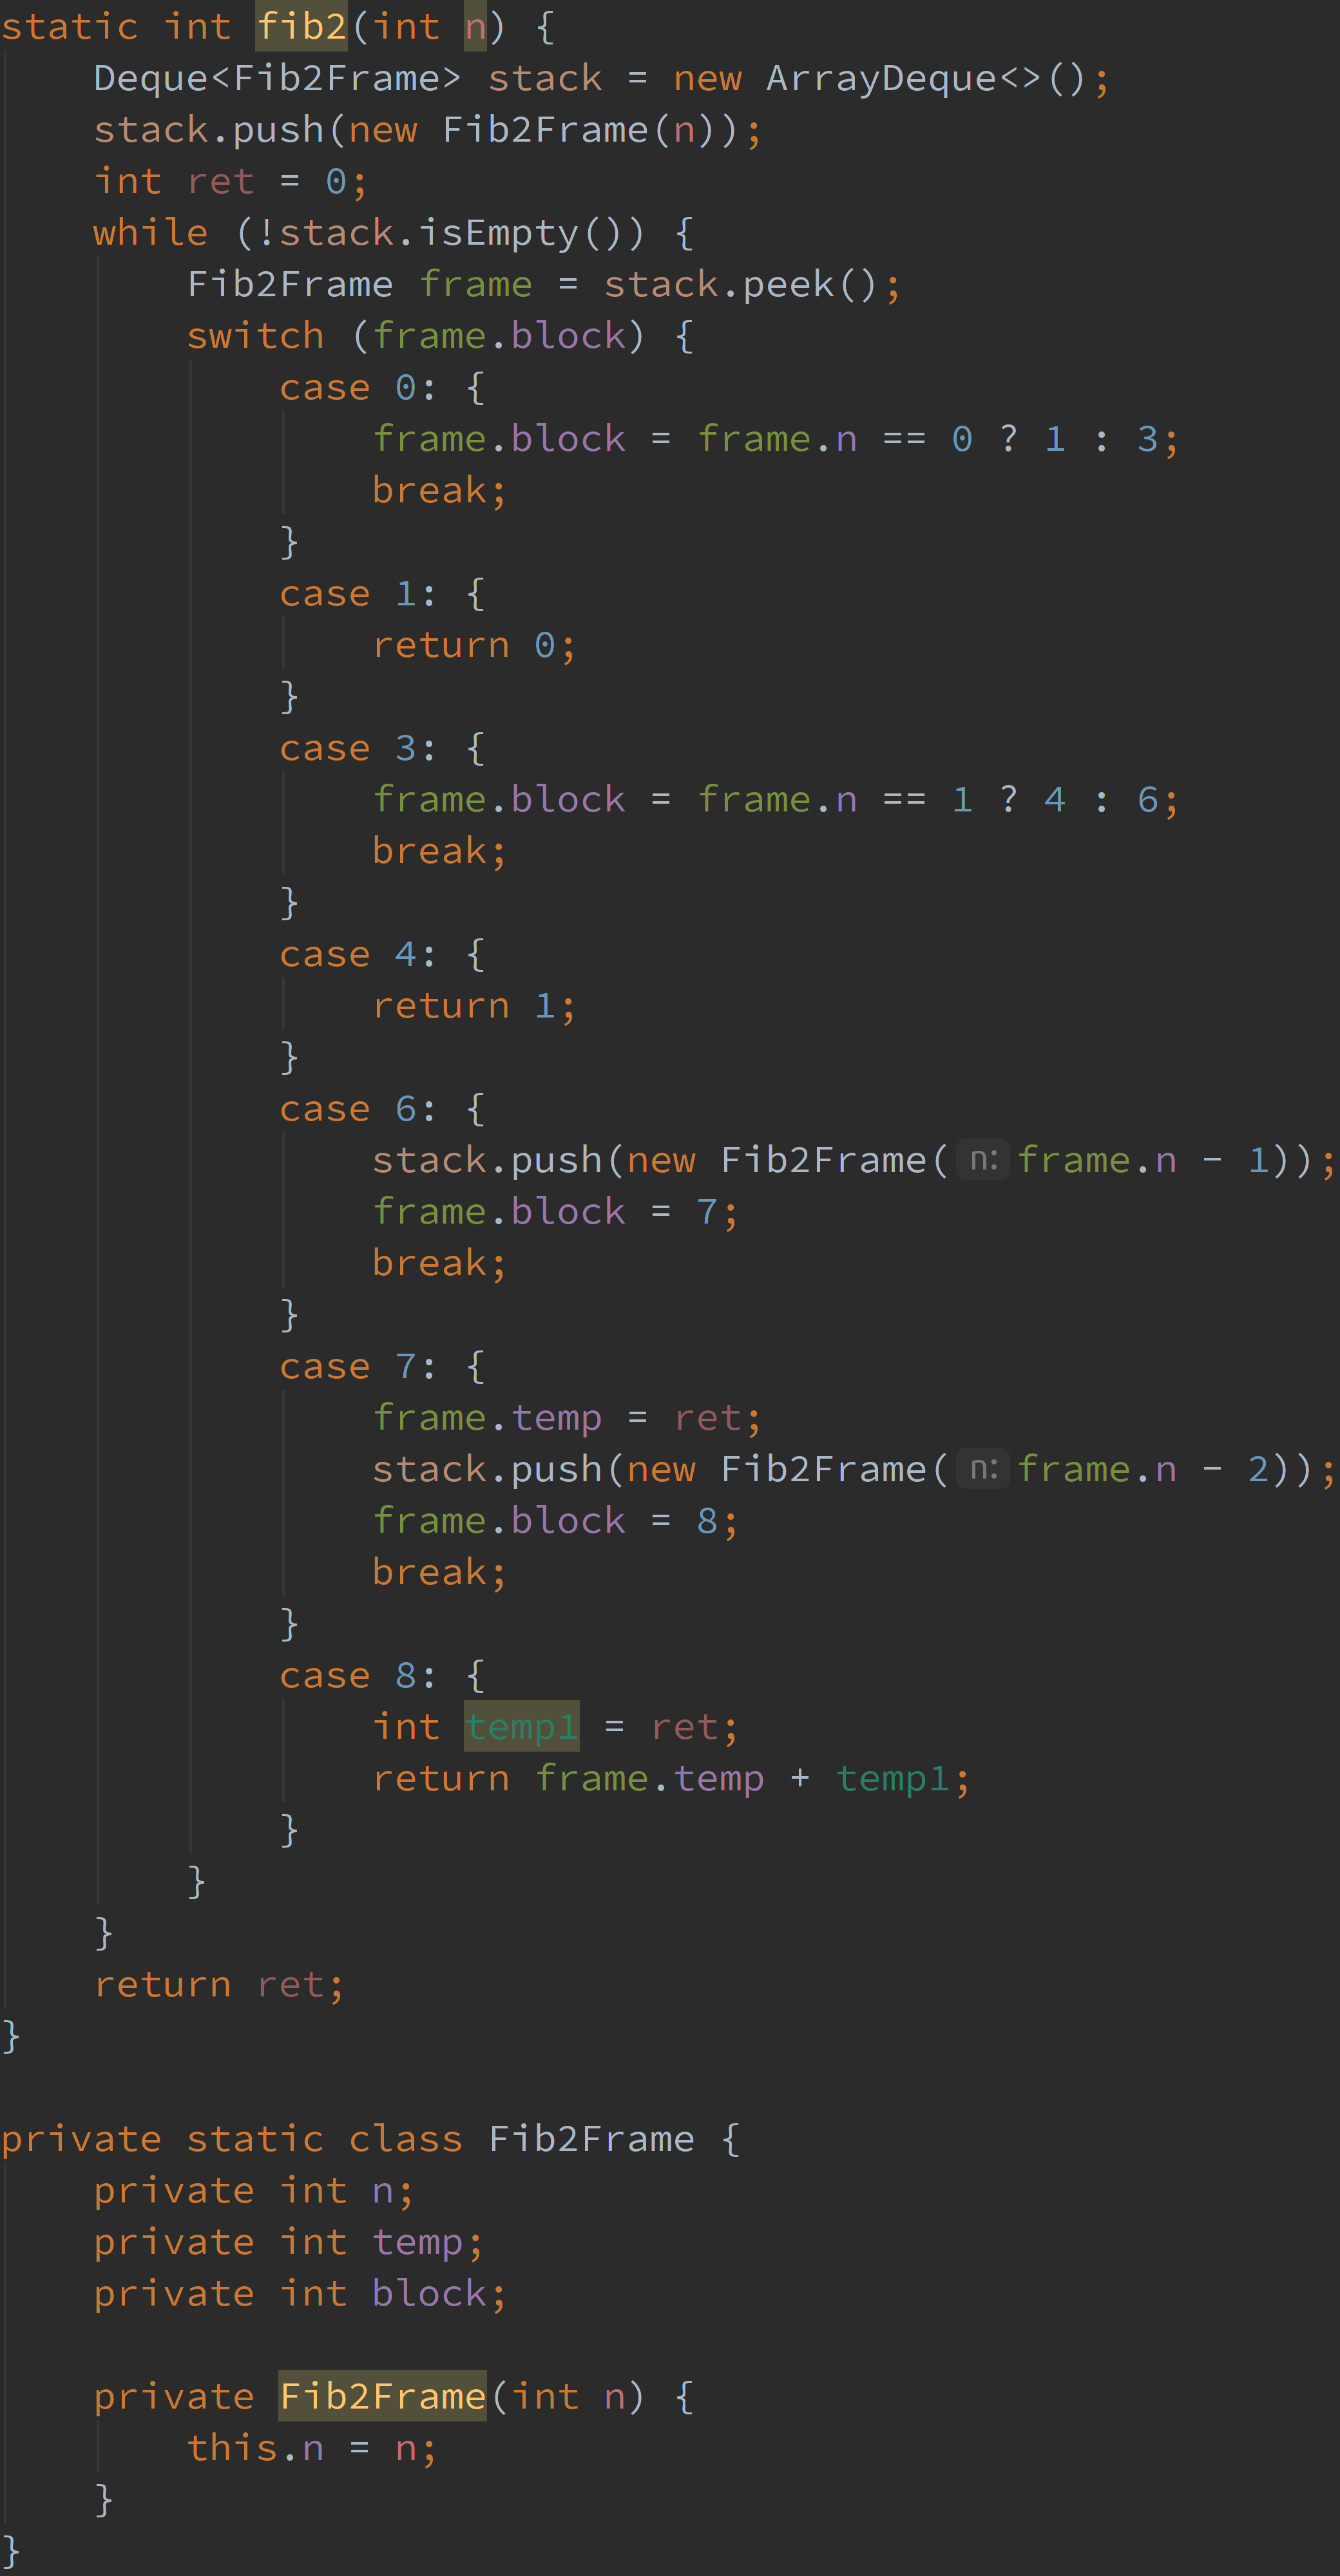
\includegraphics[height=4.464in]{src/img/remove-unreachable-after.png}
        \caption{After}
    \end{subfigure}%
    }\\
    \caption{Removing unreachable blocks \label{img:remove-unreachable}}
\end{figure}